\documentclass[12pt]{article}

\usepackage[left=1in,top=1in,right=1in,bottom=1in]{geometry}
\usepackage[utf8]{inputenc}
\usepackage[english]{babel}
\usepackage{graphicx}
\usepackage{csquotes}
\usepackage[
backend=biber,
style=chicago-authordate
]{biblatex}

\usepackage{setspace}
\doublespacing

\addbibresource{bibliography.bib}
\AtEveryBibitem{%
  \clearlist{language}%
}
 
\title{Paper Proposal for POLSCI 688}
\author{Ben Goehring}
\date{\today}

\begin{document}
\begin{titlepage}
\maketitle
\end{titlepage}

Over the last decade, state governments have passed numerous preemption laws, overturning or preventing municipalities' attempts to increase the minimum wage, ban plastic bags, prevent fracking, protect disadvantaged groups from discrimination, and enact other regulations \parencite{dupuisCityRightsEra2018,schraggerStatePreemptionLocal2017}. While states have preempted local laws in a variety of policy domains, economic regulations have garnered special attention. In the four year span from 2013 to 2017, 14 states banned localities from raising the minimum wage above the statewide wage; 17 states prevented localities from mandating employers provide some form of paid sick or family medical leave; and 11 states banned localities from requiring government contractors to pay their employees the average local wage \parencite{vonwilpertCityGovernmentsAre2017}.

The recent spate of preemption activity has generated interest among political scientists in the underlying causes of state preemption. Recent studies point to the conservatism of state legislatures \parencite{goodmanStateLegislativeIdeology2019} as well as interest group lobbying and the dominance of Republican parties in state capitals since 2010 as key causes of preemption \parencite{hicksHomeRuleBe2018,fowlerStatePreemptionLocal2019,flavinExplainingStatePreemption2019,riverstone-newellRiseStatePreemption2017}. Scholars have also found relationships between state preemption and the share of African Americans in the population \parencite{flavinExplainingStatePreemption2019} as well as between preemption and legislative professionalism, political culture, and home-rule status \parencite{fowlerStatePreemptionLocal2019}. These studies are an important first step in understanding when and why states preempt local laws. Yet, their narrow focus on post-2010 preemption activity, absence of time series analyses\footnote{For an exception, see \cite{goodmanStateLegislativeIdeology2019}.}, and lack of appreciation for the role of local action in spurring state preemption render their findings suspect.

I argue in this paper that recent state preemption must be viewed, in part, as another battle in a long-running struggle between cities and states over the bounds of local autonomy. Preemption is neither a new phenomenon nor one that can be properly understood by only studying state actions. As a historic phenomenon, one that dates back at least to battles over tobacco regulation in the 1980's, preemption deserves to be studied across a time frame wide enough to parse out whether, for instance, it is always the case that conservative Republican state governments are more likely to overturn local regulations or whether such a finding is a product of a narrow temporal scope. As another instance of cities and states struggling over how much authority cities should be able to possess, preemption needs to also be studied with an eye toward the actions of both states and cities. If preemption is a product of relations between two players - cities and states - we cannot fully understand the actions of one player without knowing the actions of the other.

The remainder of this paper is structured as follows. First, I overview the history of preemption and situate it within an even longer history of city-state relations. Second, I provide a framework for testing the underlying causes of preemption, arguing that it is most likely to occur when the probability of local action is high, organized interests are mobilized at the state level, and there is a high level of divergence between the interests of state and local policymakers. Third, I propose to test my theory using data on local policymaking and state preemption in two policy areas: the minimum wage and tobacco regulation. As high-profile issues over which cities and states have struggled for decades, the minimum wage and tobacco regulation provide plentiful variation across cities and states. I conclude by discussing some expected findings and implications from my work. 

\subsection*{History of preemption}
State interference in municipal governance dates back to the founding of the UNited States. Following the passage of the Constitution, which does not mention cities or other sub-state municipalities, state legislatures began to exert control over cities chartered in the colonial era in order to reduce local elites' authority. While state intervention was relatively rare in the first half of the 19th Century, states began to take a much more active role in municipal affairs in the latter half of the century due to economic and political pressures. The challenges wrought by urbanization and industrialization in the latter half of the century led many reformers and state legislators to see the states as having a necessary role in governing large cities while concerns over urban corruption and nativist prejudices further galvanized efforts to increase state control over city affairs (\cites[p. 53-57]{bermanLocalGovernmentStates2003}[p. 9]{kraneHomeRuleAmerica2000}). 

Rising political competition at the national and state levels also led to increased state control in the 19th Century. As party competition increased among Democrats and Republicans, state officials increasingly came to see cities as key sources of votes and patronage. As a result, municipal departments often became caught in the middle of partisan fights and were consequently transferred from city to state control -- before being transferred back to city jurisdiction when the other party gained power at the state level (\cites[p. 57-60]{bermanLocalGovernmentStates2003}[p. 11]{kraneHomeRuleAmerica2000}. Municipal employees were also often at the mercy of state officials, as their salaries and employment status could be changed without cause \parencite[p. 59]{bermanLocalGovernmentStates2003}.

Around the turn of the century, amid concerns over states' corruption and interference in city governments, progressive reformers began to push for increased local control over municipal governance. What began as a movement to stop specific state legislation targeting specific city policies, personnel, or departments grew into a larger push for increased local autonomy via Home Rule \parencite[p. 11]{kraneHomeRuleAmerica2000}. Home Rule has taken on different forms over the past century \parencite{richardsonDillonRuleMars2011}, but its early proponents emphasized that cities should, mirroring relations between the states and federal government, have a degree of immunity from state interference and possess the authority to legislate in areas of local concern (\cites[p. 11-12]{kraneHomeRuleAmerica2000}[p. 1124-1125]{dillerIntrastatePreemption2007}). By the end of the 19th Century, Missouri, California, Washington, and Minnesota had instituted Home Rule, with nine more states following suit in the first 12 years of the 20th Century \parencite[p. 11]{kraneHomeRuleAmerica2000}.

While Home Rule sought to increase cities' ability to self-govern, it was constrained by economic and legal forces. The Great Depression sharply reduced cities' revenues, leading municipalities to seek assistance from states and the federal government and place less emphasis on the independence of cities. As cities were often underrepresented at the state level (\cites{ansolabehereEndInequalityOne2008}[p. 64-67]{bermanLocalGovernmentStates2003} and slow in providing assistance, city leaders focused much of their attention on building relationships with the federal government \parencite[p. 64-65]{bermanLocalGovernmentStates2003}. The legal structure of Home Rule also reduced its impact on local autonomy. By situating municipal policymaking authority within a separate, "local" sphere, it empowered state judges to interpret the bounds of city power (\cites[p. 1125]{dillerIntrastatePreemption2007}[p. 12]{kraneHomeRuleAmerica2000}). Following the legal doctrine of Dillon's Rule, which interpreted municipal authority as only extending to the policy domains explicitly delegated by the state government, state judges often narrowly construed the bounds of cities' authority in Home Rule regimes \parencite[p. 1125]{dillerIntrastatePreemption2007}.\footnote{Dillon's Rule is named after the 19th Century jurist John Dillon. In an 1868 case in Iowa and treatise on municipal law published five years later, Dillon argued for cities to be treated as subservient to their states. "[Municipalities]," Dillon wrote, "possess no powers or faculties not conferred upon them, either expressly or by fair implication, by the law that creates them, or other statues applicable to them" \parencite[p. 93]{dillonLawMunicipalCorporations1873}. While Dillon's doctrine gained widespread traction, he was not the first to provide a legal justification for cities' subservience to states, James Kent's \textit{Commentaries on American Law}, published in 1836, argued that cities "possess subordinate legislative powers\ldots] subject to the control of the legislature of the state" \parencite[Quoted in ][p. 9]{kraneHomeRuleAmerica2000}}.





Preemption occurs when a state overturns a municipal law and/or prevents municipalities from passing legislation on a certain topic. States can preempt local laws by passing explicit legislation banning local policymaking within a certain domain or by appealing to a state court that by passing a specific law a city has overstepped its legal authority. Whether preemption occurs via legislative action or court ruling depends in part on the degree of autonomy enjoyed by cities in a state.







In the midst of these struggles over local autonomy grew a legal debate over the status of cities and how much policymaking authority they should enjoy. One one side were proponents of 




 In states that adopted Dillon's Rule, cities' policymaking authority extended only to the domains explicitly granted by the state. As Dillon wrote, "[Municipalities] possess no powers or faculties not conferred upon them, either expressly or by fair implication, by the law that creates them, or other statues applicable to them" \parencite[p. 93]{dillonLawMunicipalCorporations1873}. Dillon's notion that cities were subservient to states and could only act within explicitly defined bounds gained widespread support in the latter half of the 19th Century, providing legal justifications for state control over municipal affairs . [insert quote from plunkitt about hayseeds]

\newpage
Dillon's rule vs. Home Rule
Legal status has implications for possibility of preemption
	idea of legislatively driven preemption vs. court preemption
History of preemption 
	tobacco
	guns
	idea of "new preemption"

\newpage
\subsection*{Hypotheses}
In the prior section I discussed the history of preemption and situated it within a longer history of often tense relations between states and cities. In this section I turn to theories of when and why we should expect states to preempt local policies. I structure my discussion around three necessary conditions, arguing that a state preempts a specific type of municipal regulation when the following are met:

\singlespacing
\begin{enumerate}
	\item At least one city in the state is able to pass, or has already passed, the regulation.
	\item There is a wide divergence in policy preferences between at least one city in the state and the state.
	\item Relevant interest groups are organized at the state level. 
\end{enumerate}
\doublespacing

I hope to show that we should expect preemption to only occur when all three of these conditions are met. We should not expect to see, for instance, a state preempt a local minimum wage policy if its cities are unable to pass minimum wage legislation in the first place due to their legal status, the state shares similar policy preferences to its cities, or the state's business and industry groups are not mobilized. Instead, preemption should occur when the threat of local action is high, states and cities share different policy goals, and groups are mobilized to fight local actions. Such an expectation means that we need to heed the actions of cities, states, and interest groups. Understanding when and why preemption occurs requires factoring in all three entities' actions, preferences, and institutional contexts. In the remainder of this section, I discuss how I hope to measure these three conditions in empirical tests.

The first necessary condition in my theory of the causes of state preemption is that at least one city in the state is able to pass, or has already passed, the regulation. Cities' capacity to pass regulations depends on their legal status within their respective states. [this is where I need to discuss home rule, dillon's rule, and ideas of local autonomy see clark (1984)]

\begin{enumerate}
	\item Preemption more likely when the probability of local action is high
	\begin{enumerate}
		\item Legal stats (dillon's or home rule) (fowler and witt use krane, rigos, and hill (2001))
		\item cities have passed or are about to pass policy 
	\end{enumerate}
	\item Preemption more likely as the ideological divergence between cities and states increases
	\begin{enumerate}
		\item Republican control of state government
		\item ideological divide between state and cities (chen and rodden)
	\end{enumerate}
	\item Preemption more likely when relevant groups are organized at the state level
	\begin{enumerate}
		\item ???
	\end{enumerate}
\end{enumerate}

\begin{figure}[ht]
\caption{Number of state governments under unified partisan control, 1980-2017}
\centering
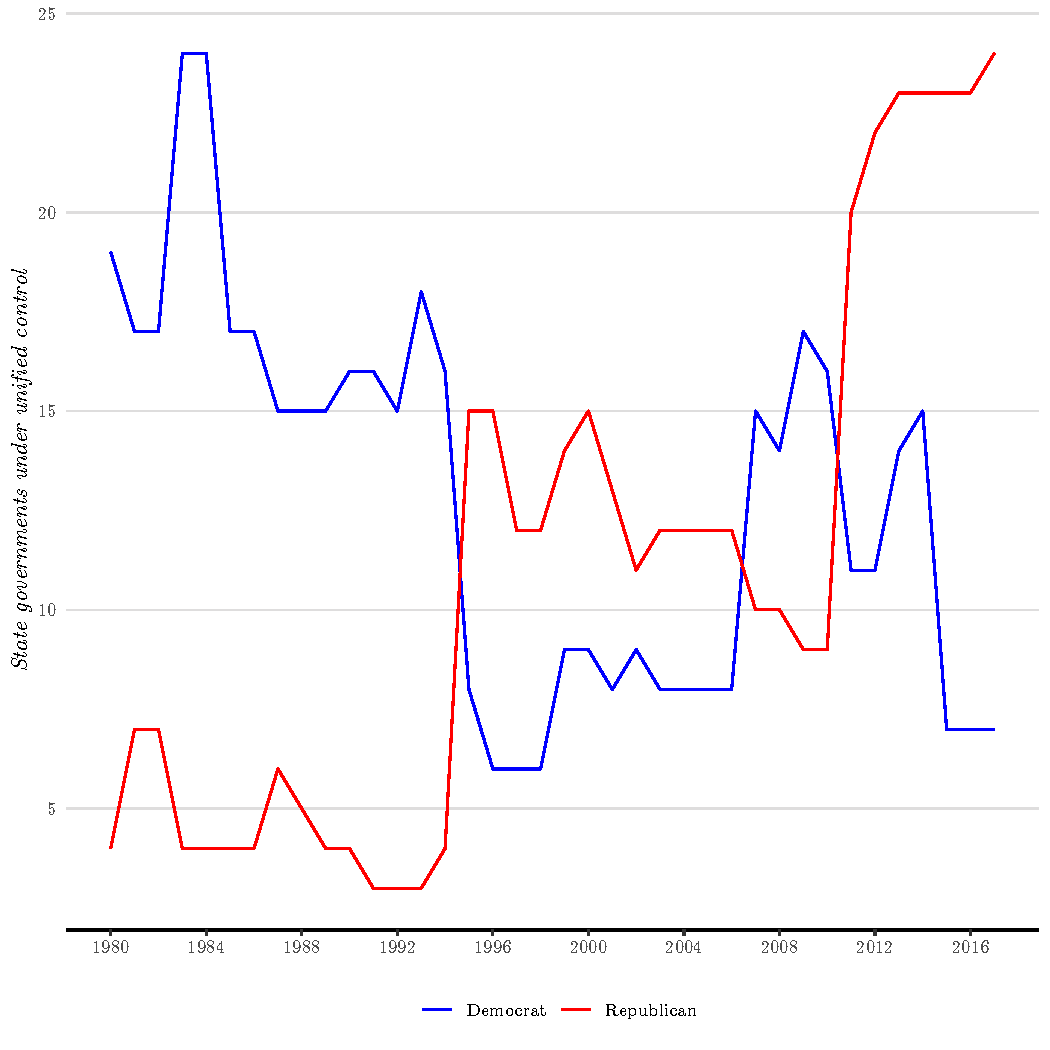
\includegraphics[width=.75\textwidth]{plots/party_control}
\end{figure}

\begin{figure}[ht]
\caption{Average relative support of Democratic presidential candidate by geography and state partisanship, 1980-2016}
\centering
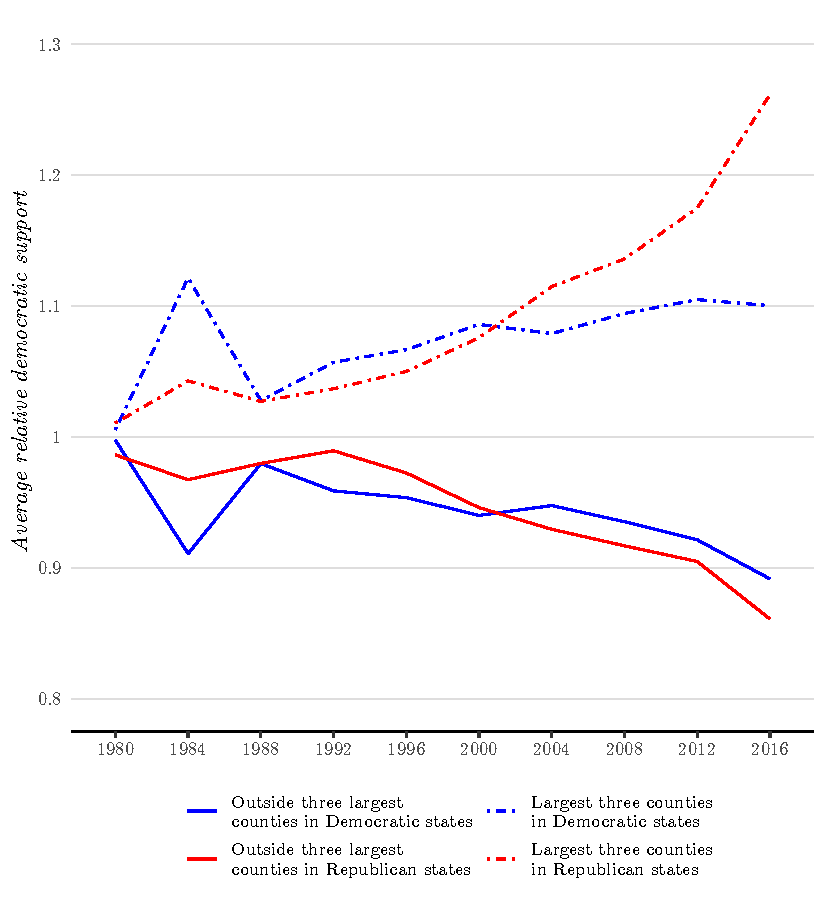
\includegraphics[width=.75\textwidth]{plots/county_support}
\end{figure}







\newpage
\printbibliography
 
\end{document}